\documentclass{scrartcl}
\usepackage{amsmath}
\usepackage{graphicx}
\usepackage{url}
\title{Cubic Interpolation with Irregularly Spaced Points}
\subtitle{Version 0.2}
\author{R. Steven Turley}
\date{August 21, 2018}
\begin{document}
\maketitle
\tableofcontents

\section{Introduction}
This is the mathematics and some implementation details
behind a derivation of 1d cubic piece-wise continuous
interpolation with regularly and irregularly spaced points.
I will explore two ways to compute this cubics: splines and
Hermite polynomials. Both are continuous and have continuous
derivatives at the knots. Splines also have continuous second
derivatives.

\section{Cubic Splines}

I will use the article on splines for a regularly-spaced
grid in MathWorld\cite{mathworld} as a basis for my
derivations and generalizations.

Splines are piece-wise cubic polynomials which are continuous
and have continuous first and second derivatives. In each interval
it takes four coefficients to define a cubic polynomial. If there
are $n+1$ points, there are $n$ intervals requiring $4n$ coefficients
for the splines. Let the knots on the spline (the data points that
match exactly) be $(x_i,y_i)$. Let $Y_i(x)$ be the cubic polynomial for
the interval $i$ where $x_i\leq x\leq x_{i+1}$. Then the $4n-4$ conditions
for matching the points and having continuous first and second derivatives
are for $2\leq n \leq n$
\begin{align}
Y_{i-1}(x_i) &= y_i \label{eq:cbegin} \\
Y_i(x_i) &= y_i\\
Y'_{i-1}(x_i) &= Y'_i(x_i)\\
Y''_{i-1}(x_i) &= Y''_i(x_i)\;. \label{eq:c2}
\end{align}
In addition to these equations, the spline also needs to match
at the two endpoints.
\begin{align}
Y_1(x_1) &= y_1\\
Y_n(x_{n+1}) &= y_{n+1}
\end{align}
This gives a total of $4n-2$ equations and $4n$ unknowns. There
are several ways to choose the last two conditions. I will use the
specification that the second derivative be zero at the two endpoints.
\begin{align}
Y''_1(x_1) &= 0 \label{eq:bslope}\\
Y''_{n+1}(x_{n+1}) &= 0 \label{eq:eslope}
\end{align}

\subsection{Regularly-Spaced Points}

The spline equations can be solved with a particularly elegant
form for the case of equally spaced knots. It is useful to put the
origin of each cubic at the beginning of the interval and transform
to a variable $t$ which goes from 0 to 1 in each interval $i$.
\begin{align}
x &= x_i + \alpha t \qquad\mbox{for}\quad x_i\leq x\leq x_{i+1}\label{eq:xt}\\
\alpha &= x_{i+1}-x_i \quad\forall i \label{eq:alpha}
\end{align}
If the
intervals are of equal length, the conditions of continuity
of a derivative with respect to $x$ is the same as a derivative
with respect to $t$. Equations~\ref{eq:cbegin} through \ref{eq:c2}
are then
\begin{align}
Y_{i-1}(1) &= y_i\\
Y_i(0) &= y_i\\
Y'_{i-1}(1) &= Y'_i(0)\\
Y''_{i-1}(1) &= Y''_i(0).
\end{align}
Let the four coefficients of the cubic for interval $i$ be given
by
\begin{equation}
Y_i(t) = a_i + b_i t + c_i t^2 + d_i t^3 .
\end{equation}
Then these coefficients can be solved for in terms of the
values $y_i$ and the derivatives $D_i = Y'_i(0)$.
\begin{align}
Y_i(0)&=y_i = a_i \label{eq:Yi0}\\
Y_i(1)&=y_{i+1} = a_i + b_i + c_i + d_i\\
Y'_i(0) &= D_i = b_i\\
Y'_i(1) &= D_{i+1} = b_i + 2 c_i + 3 d_i \label{eq:Ypi1}
\end{align}
These equations can be solved for the cubic coefficients in
terms of $y_i$ and $D_i$.
\begin{align}
a_i &= y_i \label{eq:ai}\\
b_i &= D_i\\
c_i &= 3(y_{i+1}-y_i)-2D_i-D_{i+1} \label{eq:ci}\\
d_i &= 2(y_i-y_{i+1})+D_i +D_{i+1} \label{eq:di}
\end{align}
Weisstein shows that these equations can be rewritten as
the matrix equation
\begin{equation}
\left(\begin{array}{ccccccc}
2&1\\
1&4&1\\
&1&4&1\\
&&1&4&1\\
\vdots&\ddots&\ddots&\ddots&\ddots&\ddots&\ddots\\
&&&&1&4&1\\
&&&&&1&2
\end{array}\right)
\left(\begin{array}{c}
D_1\\D_2\\D_3\\D_4\\ \vdots\\D_n\\D_{n+1}
\end{array}\right) =
\left(\begin{array}{c}
3(y_2-y_1)\\
3(y_3-y_1)\\
3(y_4-y_2)\\
\vdots\\
3(y_n-y_{n-2})\\
3(y_{n+1}-y_{n-1})\\
3(y_{n+1}-y_n)
\end{array}\right).\label{eq:eqtd}
\end{equation}
My derivation of this is in Appendix~\ref{sec:reg-deriv}.
Equation~\ref{eq:eqtd} can be solved with an efficient symmetric
tridiagonal solver in Julia for the unknown values $D_i$. Once those
are known, Equations~\ref{eq:ai} through \ref{eq:di} can be used
to solve for $a_i$, $b_i$, $c_i$, and $d_i$.

\subsection{Irregularly-Spaced Points}
If the points $x_i$ are not regularly spaced, $\alpha$ in
Equations~\ref{eq:xt} and \ref{eq:alpha} needs to be replaced
with $\alpha_i = x_{i+1}-x_i$ which will vary in each interval.
It also becomes
more sensible to define $Y_i$ as a function of $x$ instead of
a function of $t$.
\begin{equation}
Y_i(x) = a_i + b_i (x-x_i) + c_i(x-x_i)^2 + d_i (x-x_i)^3 .
\end{equation}
Letting $D_i$ be a derivative of $x$ instead of $t$,
\begin{align}
Y_i(x_i)&=y_i = a_i \label{eq:Yii}\\
Y_i(x_{i+1})&=y_{i+1} = a_i + b_i\alpha_i + c_i\alpha_i^2 + d_i\alpha_i^3\\
Y'_i(x_i) &= D_i = b_i\\
Y'_i(x_{i+1}) &= D_{i+1} =
	b_i + 2 c_i \alpha_i + 3 d_i \alpha_i^2 \label{eq:Yp1}
\end{align}
These can be solved for $a_i$, $b_i$, $c_i$ and $d_i$ as before.
\begin{align}
a_i &= y_i\\
b_i &= D_i\\
c_i &= 3\frac{y_{i+1}-y_i}{\alpha_i^2}-2\frac{D_i}{\alpha_i}-\frac{D_{i+1}}{\alpha^i} \label{eq:cirreg}\\
d_i &= 2\frac{y_i-y_{i+1}}{\alpha_i^3}+\frac{D_i}{\alpha_i^2}+\frac{D_{i+1}}{\alpha_i^2}\label{eq:dirreg}
\end{align}
With the change of variables,
the first and second derivative equations with
respect to $x$ are the same as the conditions on the
derivatives with respect to $t$.
Appendix~\ref{sec:irreg-deriv} derives the following
matrix equation as a solution for $D_i$ in terms of
$y_i$ and $\alpha_i$.
\begin{align}
\left(\begin{array}{ccccc}
2\alpha_1^{-1}&\alpha_1^{-1}\\
  \alpha_1^{-1}&2(\alpha_1^{-1}+\alpha_2^{-1})&\alpha_2^{-1}\\
 &\alpha_2^{-1}&2(\alpha_2^{-1}+\alpha_3^{-1})&\alpha_3^{-1}\\
\vdots&\ddots&\ddots&\ddots&\ddots\\
&&\alpha_{n-1}^{-1}&2(\alpha_{n-1}^{-1}+\alpha_n^{-1})&\alpha_n^{-1}\\
&&&\alpha_n^{-1}&2\alpha_n^{-1}
\end{array}\right)
\left(\begin{array}{c}
D_1\\D_2\\D_3\\ \vdots\\D_n\\D_{n+1}
\end{array}\right) =\\
\left(\begin{array}{c}
3(y_2-y_1)\alpha_1^{-2}\\
3[y_3\alpha_2^{-2}
	+y_2(\alpha_1^{-2}
	-\alpha_2^{-2})
	-y_1\alpha_1^{-2}]\\
3[y_4\alpha_3^{-2}
	+y_3(\alpha_2^{-2}
	-\alpha_3^{-2})
	-y_2\alpha_2^{-2}]\\
\vdots\\
3[y_{n+1}\alpha_n^{-2}+y_n(\alpha_{n-1}^{-2}
	-\alpha_n^{-2})-y_{n-1}\alpha_{n-1}^{-2}]\\
3(y_{n+1}-y_n)\alpha_n^{-2}
\end{array}\right).\label{eq:eqtdi}
\end{align}
% just to be safe for later

\subsection{Cubic Spline Results}
\subsubsection{Checking Validity}
Figure~\ref{fig:regSpline} is my interpolation of a spline
curve for regularly spaced points using my spline routine.
\begin{figure}
\begin{center}
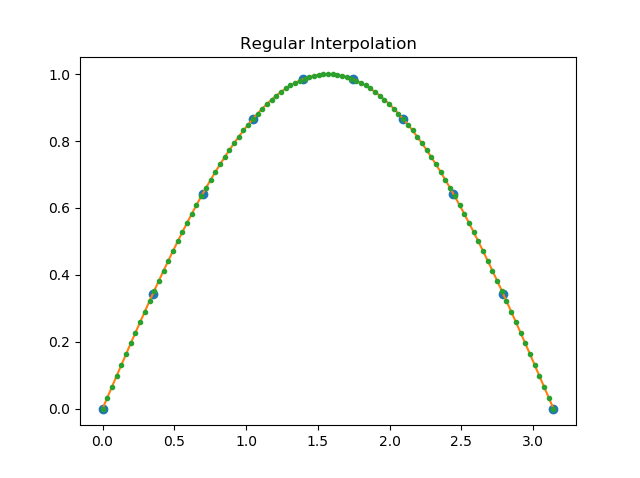
\includegraphics[width=11cm]{regSpline}
\end{center}
\caption{\label{fig:regSpline}Spline interpolation with regularly spaced
points for $\sin(x), x=0,\pi$. The large circles are the data, the dotted
line the exact curve and the orange line the spline curve.}
\end{figure}
Figure~\ref{fig:irregSpline} is the same calculation using irregularly
spaced points.
\begin{figure}
\begin{center}
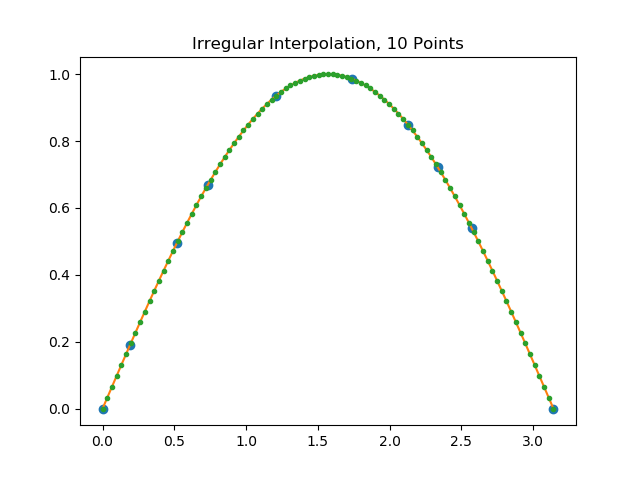
\includegraphics[width=11cm]{irregSpline}
\end{center}
\caption{\label{fig:irregSpline}Spline interpolation with irregularly
spaced points for $\sin(x), x=0,\pi$. The large circles are the data,
the dotted line the exact curve and the orange line the spline curve.}
\end{figure}
Doing the same calculation in Matlab gives similar results.
Figure~\ref{fig:matSpline} is the same calculation done in Matlab
with irregularly spaced points.
\begin{figure}
\begin{center}
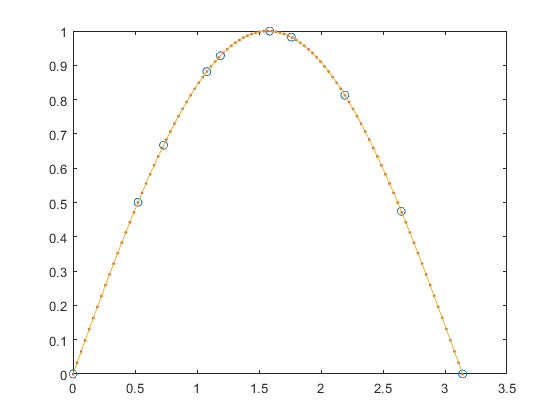
\includegraphics[width=11cm]{matSpline}
\end{center}
\caption{\label{fig:matSpline}Spline interpolation using Matlab
spline routine with irregularly spaced points.
Compare to Figure~\ref{fig:irregSpline}.}
\end{figure}
I also did a range of unit tests on the routine checking for
satisfying the spline equations and for continuity of the function
and its first two derivatives at the knots. All units tests were
passed successfully.

\subsubsection{Extra Oscillations}
If there are jumps in the data making the curve look
discontinuous, a spline can oscillate near the gap.
Consider the data in Figure~\ref{fig:csbump}
\begin{figure}
\begin{center}
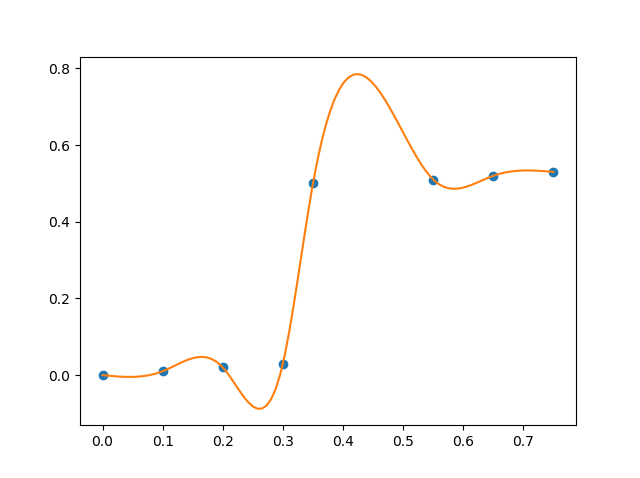
\includegraphics[width=11cm]{csbump}
\end{center}
\caption{\label{fig:csbump}Cubic spline interpolation for
data with a sudden bump.}
\end{figure}
as an example.
In this case, a piece-wise hermite polynomial
may be a better way to go. Matlab
recommends the pchip function\cite{Fritsch,Kahaner} based
on hermite polynomials to address this issue. The spline interpolation
in Matlab is identical to the Julia one. Figure~\ref{fig:pchip}
is what the pchip routine produces.
\begin{figure}
\begin{center}
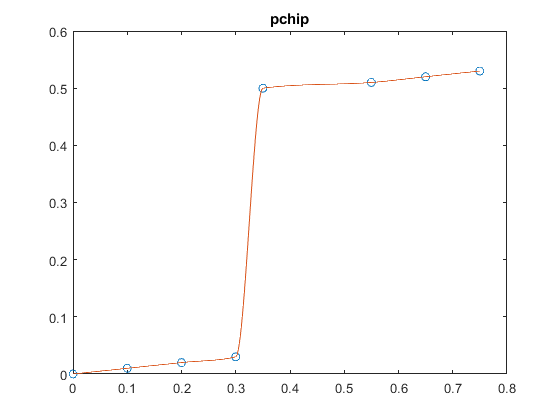
\includegraphics[width=11cm]{pchip}
\end{center}
\caption{\label{fig:pchip}Hermite polynomial interpolation
for data with a sudden bump using pchip in MATLAB.}
\end{figure}

\section{Piece-wise Hermite Polynomials}
This is probably not the most efficient implementation, but
I will follow Fritsch's notation\cite{Fritsch}
\begin{align}
f(x) &= y_i H_1(x) + y_{i+1} H_2(x) + d_i H_3(x) + d_{i+1} H_4(x)\\
y_i &= f(x_i)\\
d_i &= f'(x_i)\\
h_i &= x_{i+1}-x{i}\\
H_1(x) &= \phi\left(\frac{x{i+1}-x}{h_i}\right)\\
H_2(x) &= \phi\left(\frac{x-x_i}{h_i}\right)\\
H_3(x) &= -h_i\psi\left(\frac{x_{i+1}-x}{h_i}\right)\\
H_4(x) &= h_i\psi(\left(\frac{x-x_i}{h_i}\right)\\
\phi(t) &= 3t^2-2t^3\\
\psi(t) &= t^3-t^2
\end{align}

The prescription in Fritsch\cite{Fritsch} for producing cubic
hermite interpolants requires the derivatives at the knots. It
is not clear from the documentation which choice MATLAB
made in the pchip routine.
\subsection{Derivatives}
The formulas in the previous section require the computation of
numerical derivatives at each knot.
\subsubsection{Equally-Spaced Points}
With equally-spaced knots, this
is probably best done using the straightforward "three point formula."
\begin{equation}
y'_i \approx \frac{y_{i+1}-y_{i-1}}{2h},\label{eq:ceq}
\end{equation}
where $h=y_2-y_1=y_3-y_2$.
This formula is accurate to second order in $h$ as can be seen
from a Taylor series expansion of $f(x)$ about the point $x_i$.
\begin{equation}
f(x)=f(x_i)+f'(x_i)(x-x_i)+\frac{1}{2}f''(x_i)(x-x_i)^2+
	\frac{1}{6}f'''(x_i)(x-x_i)^3\label{eq:Taylor}
\end{equation}
Substituting Equation~\ref{eq:Taylor} into Equation~\ref{eq:ceq}
with $y_{i+1}=f(x_i+h)$, $y_{i-1}=f(x_i-h)$ and
$h=x_i-x{i-1}=x_{i+1}-x_i$ yields
\begin{equation}
y'_i=f'(x_i)=f'(x_i)+\frac{1}{6}f'''(x_i)h^2.
\end{equation}
\subsubsection{Unequally-Spaced Points}
If the points are not equally spaced, a somewhat less
accurate formula can be found from the average of the forward
and backward difference formulas.
\begin{align}
f'(x_i) &\approx \frac{f'_b(x_i)+f'_f(x_i)}{2}\\
&= \frac{y_i-y_{i-1}}{2h_b}+\frac{y_{i+1}-y_i)}{2h_f}\\
&= \frac{y_{i+1}}{2h_f}+y_i\left(\frac{1}{2h_b}-\frac{1}{2h_f}\right)
	-\frac{y_{i-1}}{2h_b} \label{eq:cuneq}\\
&= \frac{y_{i+1}}{2h_f}+y_i\frac{h_f-h_b}{2h_f h_b}
	-\frac{y_{i-1}}{2h_b}
\end{align}
where $h_f=y_{i+1}-y{i}$ and $h_b=y_i-y_{i-1}$.
Substituting the Equation~\ref{eq:Taylor} for the terms
in Equation~\ref{eq:cuneq} shows the error in this formula.
\begin{align}
\frac{f(x_{i+1})}{2h_f} &= \frac{f(x_i)}{2h_f}+\frac{f'(x_i)}{2}+
	\frac{1}{4}h_f f''(x_i)+\cdots\\
\frac{f(x_{i-1})}{2h_b} &= \frac{f(x_i)}{2h_b}-\frac{f'(x_i)}{2}+
	\frac{1}{4}h_b f''(x_i)+\cdots\\
\frac{f(x_{i+1})}{2h_f}+f(x_i)\left[\frac{1}{2h_b}-\frac{1}{2h_f}\right]
	-\frac{f(x_{i-1})}{2h_b} &= f'(x_i)+\frac{1}{4}f''(x_i)(h_f-h_b)+\cdots
\end{align}
Thus, the error in this case in linear in $h$ and proportional to
$f''(x_i)$ instead of $f'''(x_i)$ as is the case for equally spaced
points.

Another way to find a derivative is to find the quadratic polynomial
which goes through the three points and take the derivative of that.
Let
\begin{equation}
f(x)=a+b(x-x_i)+c(x-x_i)^2.
\end{equation}
At the point $f(x_{i-1}) = y_{i-1}$
\begin{equation}
y_{i-1} = a-bh_b+ch_b^2.\label{eq:ym}
\end{equation}
At the point $f(x_i)= y_i$
\begin{equation}
y_i = a. \label{eq:yi}
\end{equation}
At the point $f(x_{i+1}) = y_{i+1}$
\begin{equation}
y_{i+1} = a+bh_f+ch_f^2.\label{eq:yp}
\end{equation}
Substituting Equation~\ref{eq:yi} into Equation~\ref{eq:ym}
and Equation~\ref{eq:yi}, solving the remaining equations for $c$
and then equating them to solve for $b$ yields
\begin{equation}
b = f'(x_i) = \frac{(y_i-y{i-1})h_f}{h_b(h_f+h_b)}+
	\frac{(y_{i+1}-y{i})h_b}{h_f(h_f+h_b)}.
\end{equation}

\appendix
\section{Spline Solution for Regularly-Spaced Points}\label{sec:reg-deriv}
The goal is to solve Equations~\ref{eq:Yi0} through \ref{eq:Ypi1}
by eliminating the cubic coefficients and only having equations
in terms of the $y_i$ and $D_i$ variables. We first need to
add two more equations.
\begin{align}
Y''_i(0) &= 2c_i\label{eq:ypp0}\\
Y''_i(1) &= Y''_{i+1}(0) = 2c_i+6d_i\label{eq:yppn}\\
c_{i+1} &= c_i + 3d_i. \label{eq:cd}
\end{align}
Substituting in the values for $c_i$ from Equation~\ref{eq:ci} and
$d_i$ from Equation~\ref{eq:di}, Equation~\ref{eq:cd} becomes
\begin{multline}
3(y_{i+2}-y_{i+1})-2D_{i+1}-D_{i+2} = 3(y_{i+1}-y_i)-2D_i-D_{i+1}\\
	+3[2(y_i-y_{i+1})+D_i+D_{i+1}].
\end{multline}
Grouping the $y$ variables on one side of the equation and the $D$
variables on the other,
\begin{equation}
3(y_{i+2}-y_i) = D_{i+2} +4D{i+1} +D_i.
\end{equation}
This accounts for the middle rows of Equation~\ref{eq:eqtd}. The
top and bottom rows come from the initial and final conditions
in Equations~\ref{eq:bslope} and \ref{eq:eslope}. Combining
Equations~\ref{eq:bslope}, \ref{eq:ypp0}, and \ref{eq:ci},
\begin{align}
2c_1 & = 0\\
3(y_2-y_1) &= 2D_1 + D_2,
\end{align}
which is the first row of Equation~\ref{eq:eqtd}. Combining
Equations~\ref{eq:eslope}, \ref{eq:yppn}, \ref{eq:ci}, and
\ref{eq:di},
\begin{align}
2c_n+6d_n &= 0\\
3(y_{n+1}-y_n)-2D_n-D_{n+1}+3[2(y_n-y_{n+1})+D_n+D_{n+1}] &= 0\\
3(y_n-y_{n+1}) &= D_n+2D_{n+1},
\end{align}
which is the bottom row of Equation~\ref{eq:eqtd}.

\section{Spline Solution for Irregularly-Spaced Points}\label{sec:irreg-deriv}
The goal is to solve Equations~\ref{eq:Yi0} through \ref{eq:Ypi1}
by eliminating the cubic coefficients and only having equations
in terms of the $y_i$, $D_i$, and $\alpha_i$ variables.
We first need to add two more equations.
\begin{align}
Y''_i(x_i) &= 2c_i\label{eq:ypp0i}\\
Y''_i(x_{i+1}) &= Y''_{i+1}(x_{i+1})
 = 2c_i+6d_i\alpha_i\label{eq:yppni}\\
c_{i+1} &= c_i + 3d_i \alpha_i. \label{eq:cdi}
\end{align}
Substituting in the values for $c_i$ from Equation~\ref{eq:cirreg} and
$d_i$ from Equation~\ref{eq:dirreg}, Equation~\ref{eq:cdi} becomes
\begin{multline}
3\frac{y_{i+2}-y_{i+1}}{\alpha_{i+1}^2}-2\frac{D_{i+1}}{\alpha_i}
	-\frac{D_{i+2}}{\alpha_{i+1}} = \\
	3\frac{y_{i+1}-y_i}{\alpha_i^2}-2\frac{D_i}{\alpha_i}
	-\frac{D_{i+1}}{\alpha_i}
	+3\left[2\frac{y_i-y_{i+1}}{\alpha_i^2}+\frac{D_i}{\alpha_i}
	+\frac{D_{i+1}}{\alpha_i}\right].
\end{multline}
Grouping the $y$ variables on one side of the equation and the $D$
variables on the other,
\begin{equation}
3\left[\frac{y_{i+2}}{\alpha_{i+1}^2}+y_{i+1}\left(\frac{1}{\alpha_i^2}
	-\frac{1}{\alpha_{i+1}^2}\right)-\frac{y_i}{\alpha_i^2}\right]
	= \frac{D_{i+2}}{\alpha_{i+1}}
		+2D_{i+1}\left(\frac{1}{\alpha_i}+\frac{1}{\alpha_{i+1}}\right)
		+\frac{D_i}{\alpha_i}.
\end{equation}
This accounts for the middle rows of Equation~\ref{eq:eqtdi}. The
top and bottom rows come from the initial and final conditions
in Equations~\ref{eq:bslope} and \ref{eq:eslope}. Combining
Equations~\ref{eq:bslope}, \ref{eq:ypp0i}, and \ref{eq:cirreg},
\begin{align}
2c_1 & = 0\\
3\frac{(y_2-y_1)}{\alpha_1^2} &= 2\frac{D_1}{\alpha_1} + \frac{D_2}{\alpha_1},
\end{align}
which is the first row of Equation~\ref{eq:eqtdi}. Combining
Equations~\ref{eq:eslope}, \ref{eq:yppni}, \ref{eq:cirreg}, and
\ref{eq:dirreg},
\begin{align}
2c_n+6d_n\alpha_n &= 0\\
3\frac{y_{n+1}-y_n}{\alpha_n^2}-2\frac{D_n}{\alpha_n}
	-\frac{D_{n+1}}{\alpha_n}
	+3\left[2\frac{y_n-y_{n+1}}{\alpha_n^2}+\frac{D_n}{\alpha_n}
	+\frac{D_{n+1}}{\alpha_n}\right] &= 0\\
3\frac{y_n-y_{n+1}}{\alpha_n^2} &= \frac{D_n}{\alpha_n}
	+2\frac{D_{n+1}}{\alpha_n},
\end{align}
which is the bottom row of Equation~\ref{eq:eqtd}.

\begin{thebibliography}{9}

\bibitem{mathworld}
Weisstein, Eric W. "Cubic Spline." From
\textit{MathWorld}--A Wolfram Web Resource.
\url{http://mathworld.wolfram.com/CubicSpline.html} (accessed
8/17/2018). Citing: Bartels, R. H.; Beatty, J. C.; and Barsky, B. A.
"Hermite and Cubic Spline Interpolation," Ch. 3 in
\textit{An Introduction to Splines for Use in Computer Graphics
and Geometric Modelling}. San Francisco, CA: Morgan Kaufmann,
pp. 9--17, 1998.

\bibitem{Fritsch}
Fritsch, F. N. and R. E. Carlson. "Monotone Piecewise Cubic Interpolation." SIAM Journal on Numerical Analysis. Vol. 17, 1980, pp.238-–246.

\bibitem{Kahaner}
Kahaner, David, Cleve Moler, Stephen Nash. Numerical Methods and Software. Upper Saddle River, NJ: Prentice Hall, 1988.

\end{thebibliography}

\end{document}
